%%%%%%%%%%%%%%%%%%%%%%%%%%%%%%%%%%%%%%%%%
% Structured General Purpose Assignment
% LaTeX Template
%
% This template has been downloaded from:
% http://www.latextemplates.com
%
% Original author:
%  Ted Pavlic (http://www.tedpavlic.com)
% Modified by:
%  Joe Del Rocco (https://joe.delrocco.org)
%%%%%%%%%%%%%%%%%%%%%%%%%%%%%%%%%%%%%%%%%

%----------------------------------------------------------------------------------------
%  PACKAGES AND CONFIGURATION
%----------------------------------------------------------------------------------------

\documentclass[fleqn]{article}
\usepackage{geometry}
\usepackage{fancyhdr} % For custom headers
\usepackage{lastpage} % To determine the last page for the footer
\usepackage{extramarks} % For headers and footers
\usepackage[most]{tcolorbox} % For problem answer sections
\usepackage{graphicx} % For inserting images
\usepackage{xcolor} % For link coloring
\usepackage[hidelinks]{hyperref} % For URL links (no box or color name)
\usepackage{bm}
\usepackage{amsmath}
\usepackage{amssymb}


% Margins
\geometry{
a4paper,
tmargin=1in,
bmargin=1in,
lmargin=1in,
rmargin=1in,
textwidth=6.5in,
textheight=9.0in,
headsep=0.25in
}

% Header and footer
\pagestyle{fancy}
\lhead{\myName} % Top left header
\chead{\myCourse: \myAssignment} % Top center header
\rhead{\firstxmark} % Top right header
\lfoot{\lastxmark} % Bottom left footer
\cfoot{} % Bottom center footer
\rfoot{Page\ \thepage\ of\ \pageref{LastPage}} % Bottom right footer
\renewcommand\headrulewidth{0.4pt} % Size of the header rule
\renewcommand\footrulewidth{0.4pt} % Size of the footer rule

% Other configurations
\setlength\parindent{0pt} % Removes all indentation from paragraphs
\setlength\parskip{1pt} % Ensures paragraphs are still recognizable as such
\setcounter{secnumdepth}{0} % Removes default section numbers
\setcounter{tocdepth}{3} % Sets depth of table of contents
\linespread{1.1}

% Template values
\newcommand{\myLogo}{starfleet.jpg}
\newcommand{\myName}{Manish Yadav}
\newcommand{\myJobTitle}{3836-6483}
\newcommand{\myCompany}{Starfleet Academy}
\newcommand{\myLocation}{1701 Lincoln Blvd, San Francisco, CA}
\newcommand{\myURL}{www.starfleet.edu}
\newcommand{\myEmail}{m.yadav@ufl.edu}
\newcommand{\myCourse}{CNT5106C}
\newcommand{\mySection}{Fall 2020}
\newcommand{\myTeacher}{Dr. Ye Xia}
\newcommand{\myAssignment}{Homework 1}
\newcommand{\myDueDate}{Tue,\ Sept\ 15,\ 2020}
\newcommand{\norm}[1]{\left\lVert#1\right\rVert}


%----------------------------------------------------------------------------------------
%  DOCUMENT STRUCTURE (MACROS & ENVIRONMENTS)
%----------------------------------------------------------------------------------------

% Colored links macro
\newcommand{\hrefcol}[3] {\href{#1}{\textcolor{#3}{#2}}}

% Creates a counter to keep track of the number of problems
\newcounter{homeworkProblemCounter}

% Macro for custom title page signature header
\newsavebox{\myTitleSignature}
\sbox{\myTitleSignature}{%
\begin{tabular*}{\textwidth}{@{}l@{}@{\extracolsep{0.125in}}l@{}}%
\parbox[c][]{2.5in}{{\textbf{\myName} \par}
                    {\small \myJobTitle \par}
                    {\small \hrefcol{mailto:\myEmail}{\myEmail}{blue}} \par}
\end{tabular*}}

% Header and footer for when a page split occurs within a problem environment
\newcommand{\enterProblemHeader}[1]{%
\nobreak\extramarks{#1}{#1 continued on next page\ldots}\nobreak%
\nobreak\extramarks{#1 (continued)}{#1 continued on next page\ldots}\nobreak%
}

% Header and footer for when a page split occurs between problem environments
\newcommand{\exitProblemHeader}[1]{%
\nobreak\extramarks{#1 (continued)}{#1 continued on next page\ldots}\nobreak%
\nobreak\extramarks{#1}{}\nobreak%
}

\newcommand{\homeworkProblemName}{} % Argument = name of problem; default = "Problem #"
\newenvironment{homeworkProblem}[1][Problem \arabic{homeworkProblemCounter}]{%
\stepcounter{homeworkProblemCounter}% % Increase counter for number of problems
\renewcommand{\homeworkProblemName}{#1}% % Assign \homeworkProblemName the argument
\section{\homeworkProblemName}% % Make a section in the document with the custom problem count
\enterProblemHeader{\homeworkProblemName}% % Header and footer within environment
}{%
\exitProblemHeader{\homeworkProblemName}% % Header and footer after environment
}

\newcommand{\problemAnswer}[1]{ % Defines the problem answer command with the content as the only argument
\begin{tcolorbox}[breakable,enhanced,colback=gray!5!white,title=Answer]%
#1
\end{tcolorbox}%
% Alternative - Makes the box around the problem answer and puts the content inside
%\noindent\framebox[\columnwidth][c]{\begin{minipage}{0.98\columnwidth}#1\end{minipage}}
}

\newcommand{\homeworkSectionName}{}
\newenvironment{homeworkSection}[1]{% % For sections w/in problems; Argument = name of section (no default)
\renewcommand{\homeworkSectionName}{#1}% % Assign \homeworkSectionName the argument
\subsection{\homeworkSectionName}% % Make a subsection with the name of the subsection
\enterProblemHeader{\homeworkProblemName\ [\homeworkSectionName]}% % Header and footer within environment
}{%
\enterProblemHeader{\homeworkProblemName}% % Header and footer after environment
}

%----------------------------------------------------------------------------------------
%   TITLE PAGE
%----------------------------------------------------------------------------------------
\begin{document}

% Blank out the traditional title page
\title{\vspace{-1in}} % no title name
\author{} % no author name
\date{} % no date listed
\maketitle % makes this a title page

% Use custom title macro instead
\usebox{\myTitleSignature}
\vspace{1in} % spacing below title header

% Assignment title
{\centering \huge \myAssignment \par}
{\centering \noindent\rule{4in}{0.1pt} \par}
\vspace{0.05in}
{\centering \myCourse~: \mySection~: \myTeacher \par}
{\centering Due \myDueDate \par}
%{\centering Prepared w/ \LaTeX \par}
\vspace{1in}

% Table of Contents
\tableofcontents
\newpage

%----------------------------------------------------------------------------------------
%	PROBLEM 1
%----------------------------------------------------------------------------------------

%\begin{homeworkProblem}[Exercise \#\arabic{homeworkProblemCounter}] % Use for custom section title
\begin{homeworkProblem}
\begin{homeworkSection}{(a)}
\problemAnswer{
The transmission delay is L/R and is the amount of time required to push all of the packet's bit into the link.

\begin{equation}
    d_{trans} = \frac{1KB \times 8 \mbox{ bits/byte}}{1 \mbox{Mbps}} = 8ms
\end{equation}

The amount of required to propagate from one link to another is using propagation delay

\begin{equation}
    d_{prop} = \frac{100Km}{20000 Km/s} = 5ms
\end{equation}

The processing time at each router is $5\mu s$

In order to calculate total end to end delay is given using
\begin{align*}
    d_{end-to-end} &= 3 * d_{trans} + 3 * d_{prop} + 2 * d_{proc} \\
    & = 3 * 8 + 3 * 5 + 2 * 0.005 \\
    & = 39.01ms
\end{align*}
}
\end{homeworkSection}
\begin{homeworkSection}{(b)}
\problemAnswer{
In case of cut-through, router does not wait for the entire packet to arrive. Therefore there would no transmission delay. In order to solve this, the equation in (a) could be transformed as

\begin{align*}
    d_{end-to-end} &= d_{trans} + 3 * d_{prop} + 2 * d_{proc} \\
    & = 8 + 3 * 5 + 2 * 0.005 \\
    & = 23.01ms
\end{align*}
}
\end{homeworkSection}

\begin{homeworkSection}{(c)}
\problemAnswer{
Since $R_1 = R_2 = R_3 = 1Gbps$, the new transmission delay is 

\begin{equation}
    d_{trans} = \frac{1KB \times 8 \mbox{ bits/byte}}{1 \mbox{Gbps}} = 8\mu s
\end{equation}

In case of store and forward, 
\begin{align*}
    d_{end-to-end} &= d_{trans} + 3 * d_{prop} + 2 * d_{proc} \\
    & = 3 * 0.008 + 3 * 5 + 2 * 0.005 \\
    & = 15.034ms
\end{align*}

In case of cut through, 
\begin{align*}
    d_{end-to-end} &= d_{trans} + 3 * d_{prop} + 2 * d_{proc} \\
    & =  0.008 + 3 * 5 + 2 * 0.005 \\
    & = 15.018ms
\end{align*}
}
\end{homeworkSection}


\begin{homeworkSection}{(d)}
\problemAnswer{
\begin{align*}
    d_{trans}^{R_1,R_2} = \frac{1KB \times 8 \mbox{ bits/byte}}{2 \mbox{Mbps}} = 4ms
\end{align*}

\begin{align*}
    d_{trans}^{R_3} = \frac{1KB \times 8 \mbox{ bits/byte}}{1 \mbox{Mbps}} = 8ms
\end{align*}

In case of \textbf{store and forward}, \\
For packet 1:
\begin{align*}
    d_{end-to-end} = 2 * 4 + 8 + 3 * 5 = 31ms
\end{align*}

In case of packet 2, packet 1 is still being served \\
\begin{align*}
    d_{end-to-end} = 31 + 4 = 35ms
\end{align*}

In case of packet 3, packet 2 is still being served \\
\begin{align*}
    d_{end-to-end} = 31 + 8 = 39ms
\end{align*}

In case of \textbf{cut through}, \\
For packet 1:
\begin{align*}
    d_{end-to-end} = 3 * 5 + 8 = 23ms
\end{align*}

In case of packet 2, \\
\begin{align*}
    d_{end-to-end} = 23 + 4 = 27ms
\end{align*}

In case of packet 3,  \\
\begin{align*}
    d_{end-to-end} = 27 + 4 = 31ms
\end{align*}

}
\end{homeworkSection}


\begin{homeworkSection}{(e)}
\problemAnswer{
            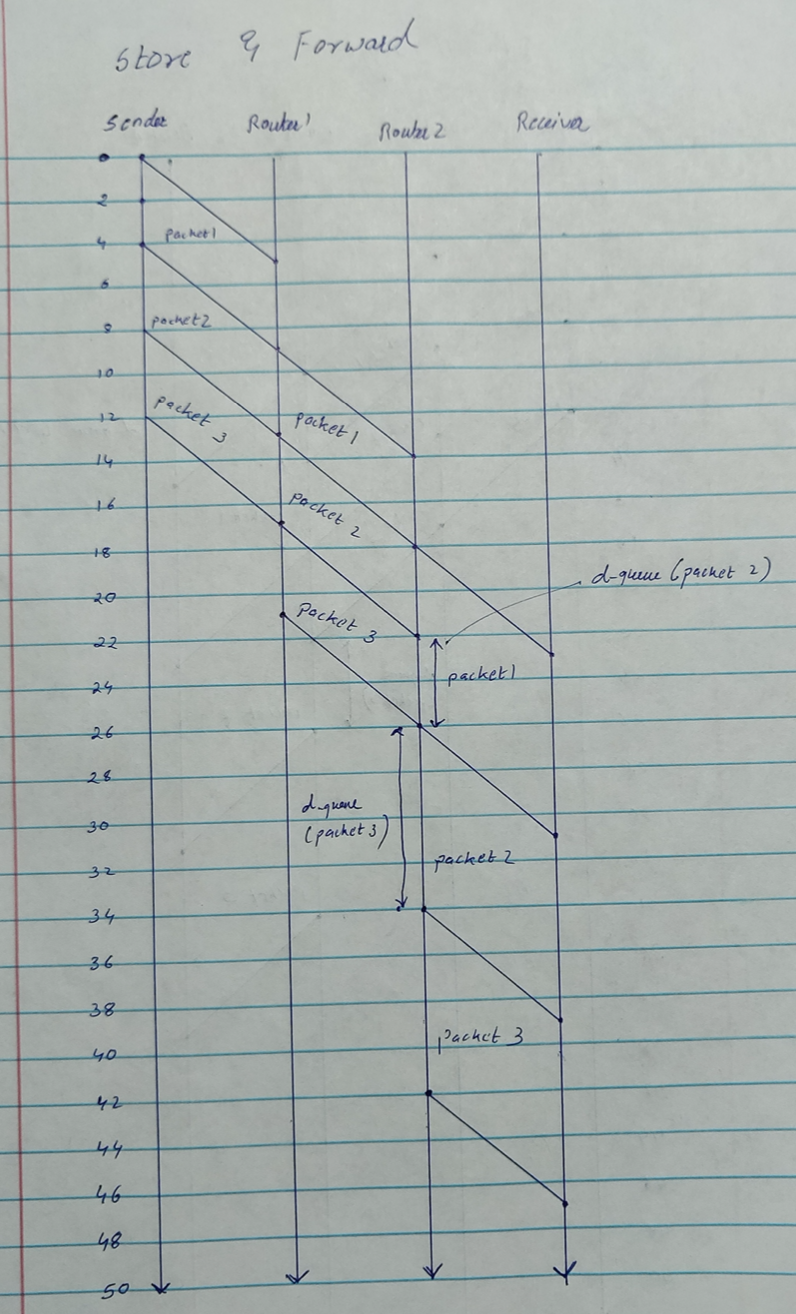
\includegraphics[width=0.75\columnwidth]{snf.png}
            \vspace{2mm}
            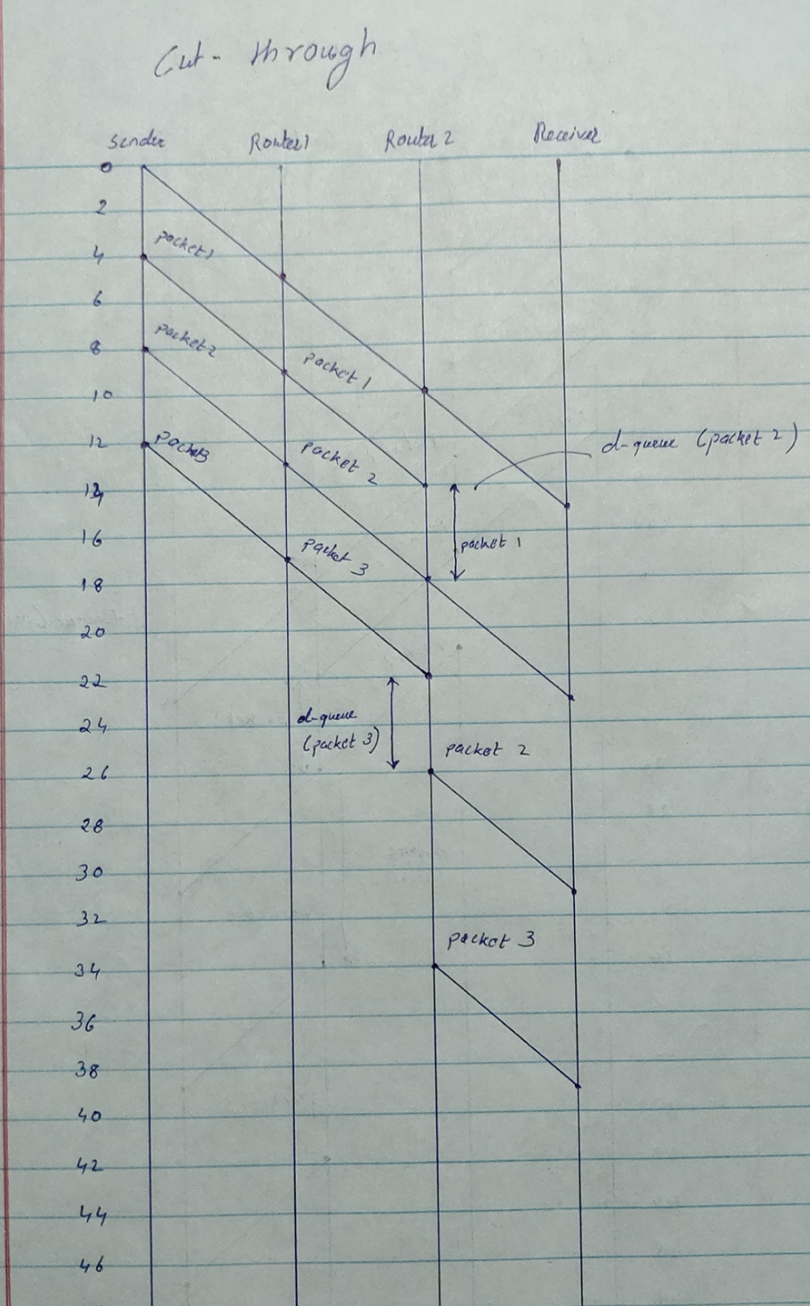
\includegraphics[width=0.75\columnwidth]{ct.png}
}
\end{homeworkSection}
\end{homeworkProblem}
%----------------------------------------------------------------------------------------
\pagebreak

\begin{homeworkProblem}
\begin{homeworkSection}{(a)}

\problemAnswer{
    \begin{center}
            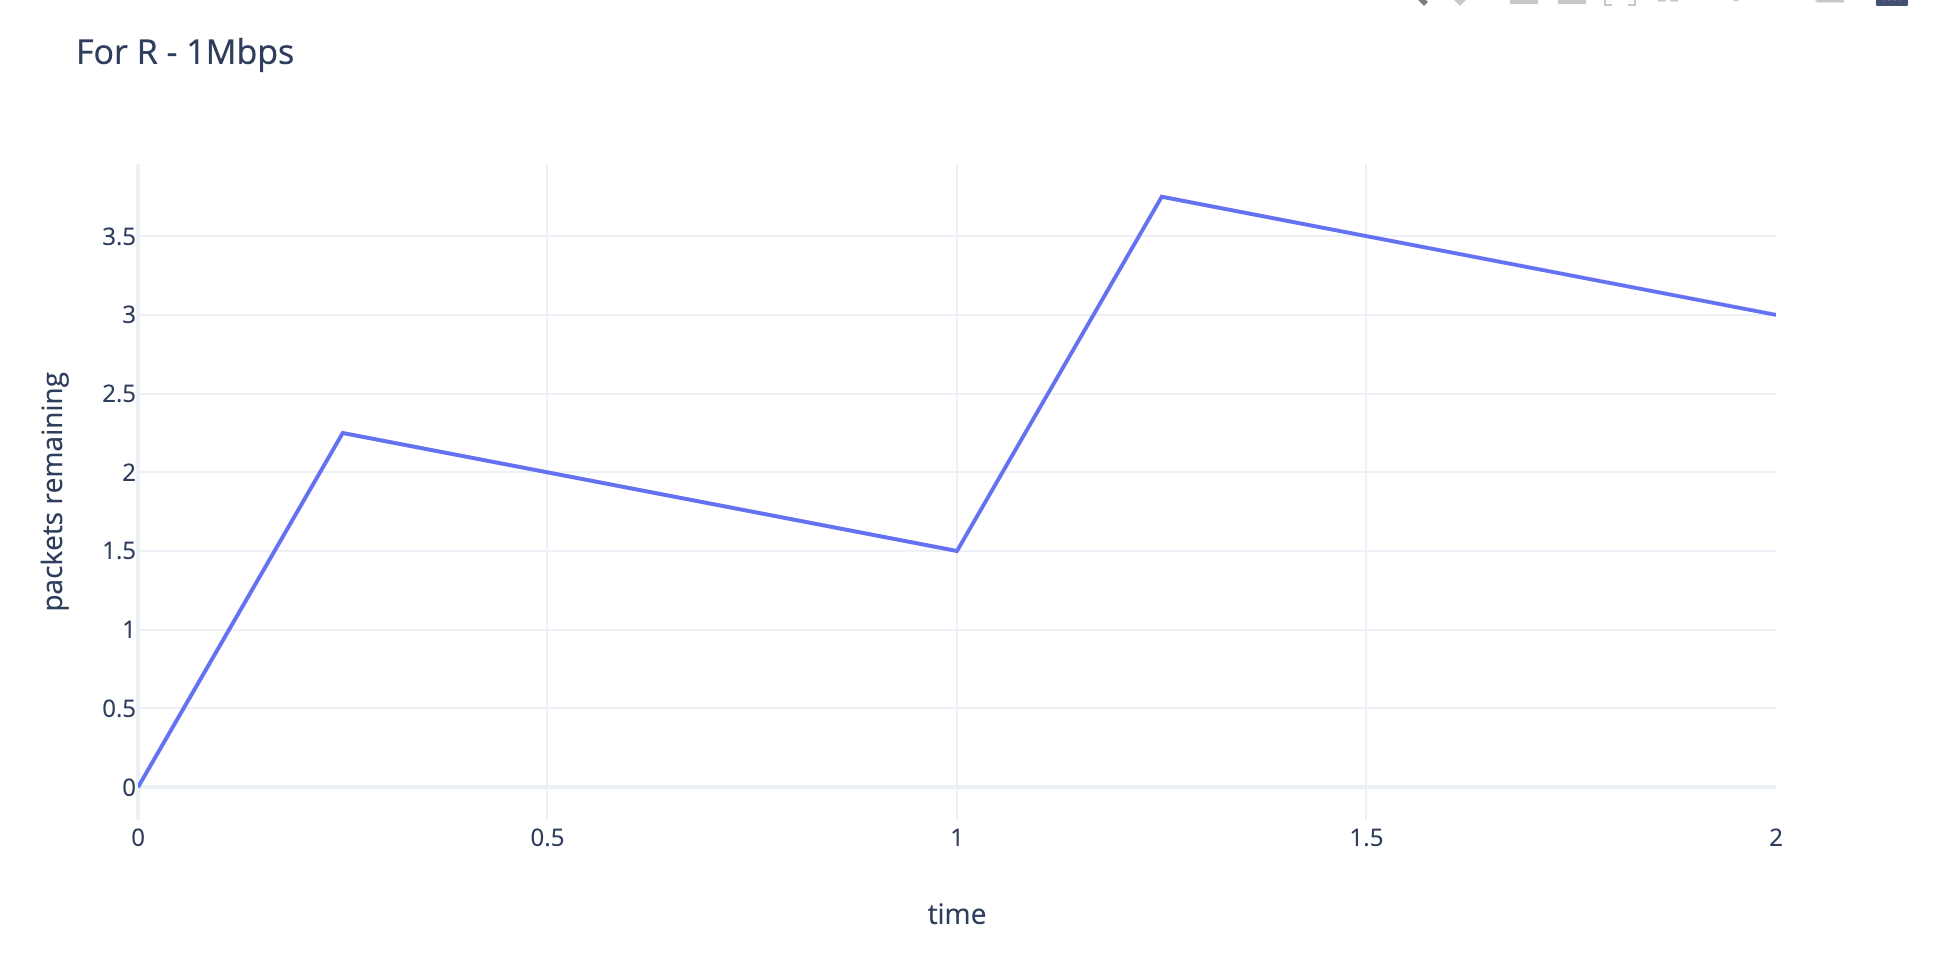
\includegraphics[width=0.75\columnwidth]{1.png}
            
            \vspace{2mm}
            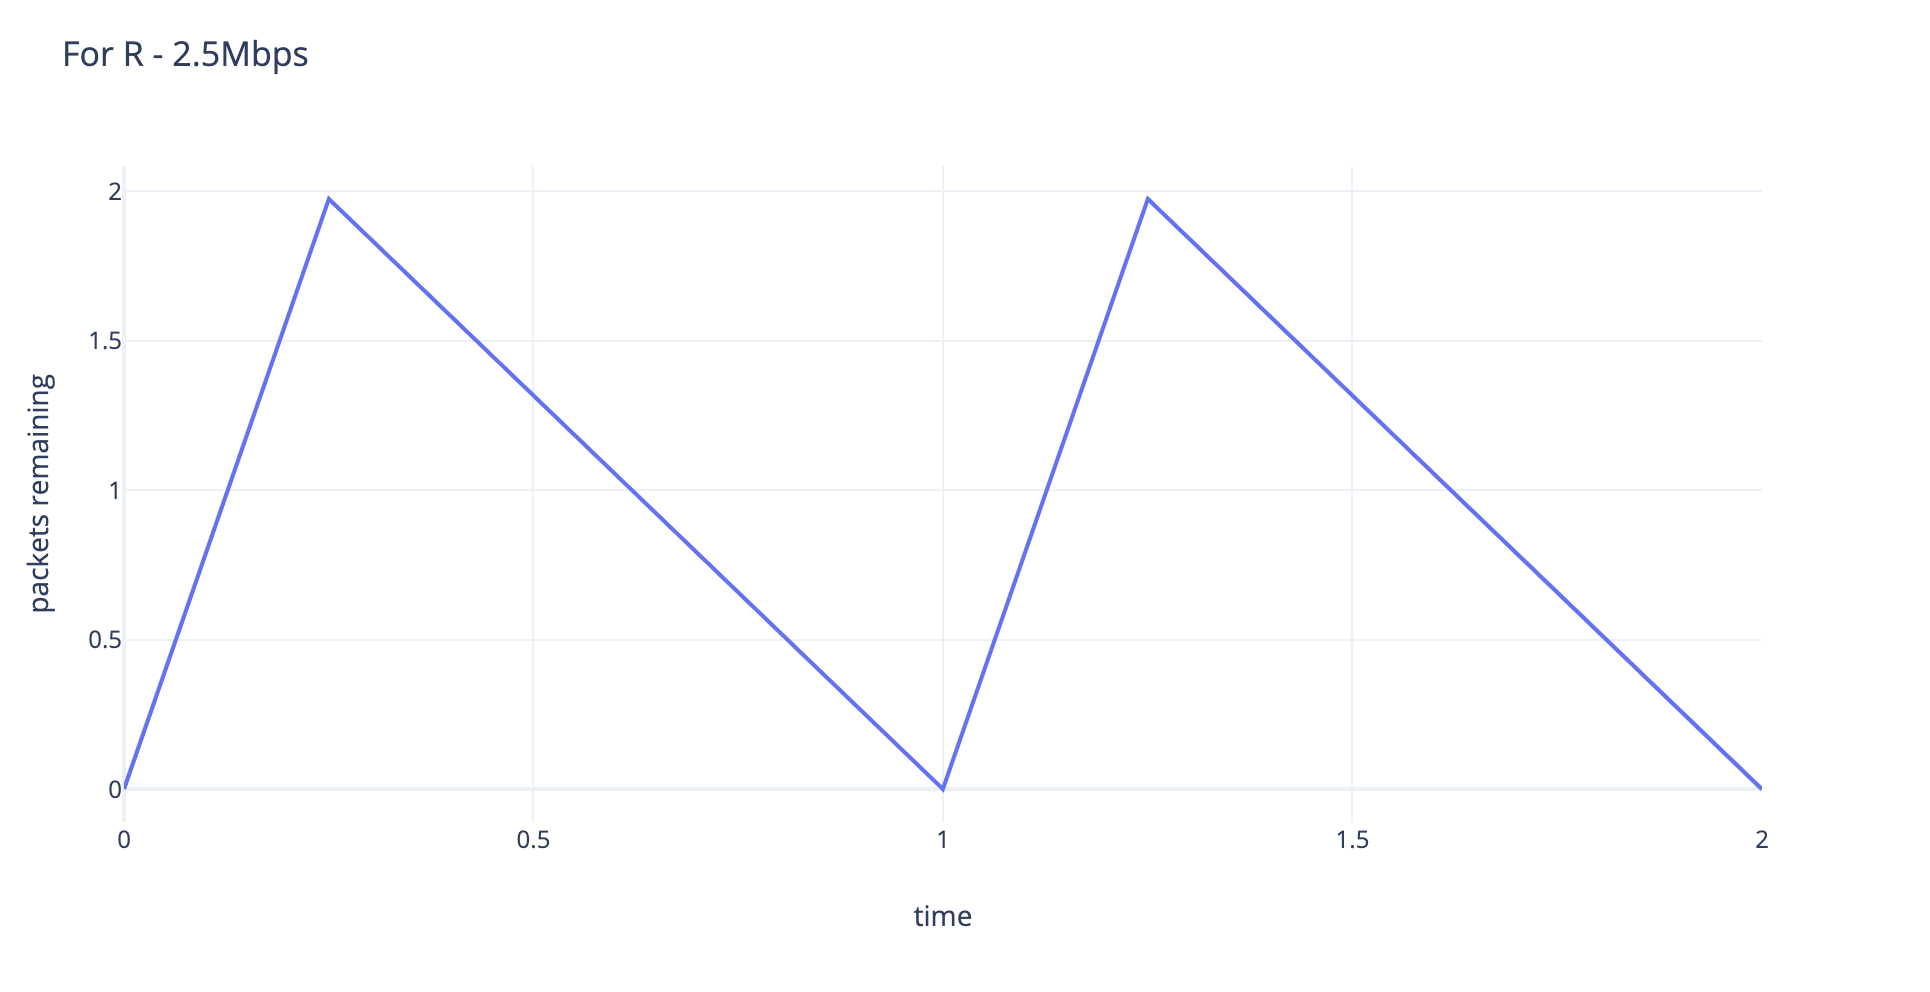
\includegraphics[width=0.75\columnwidth]{r_25.png}
            
            \vspace{2mm}
            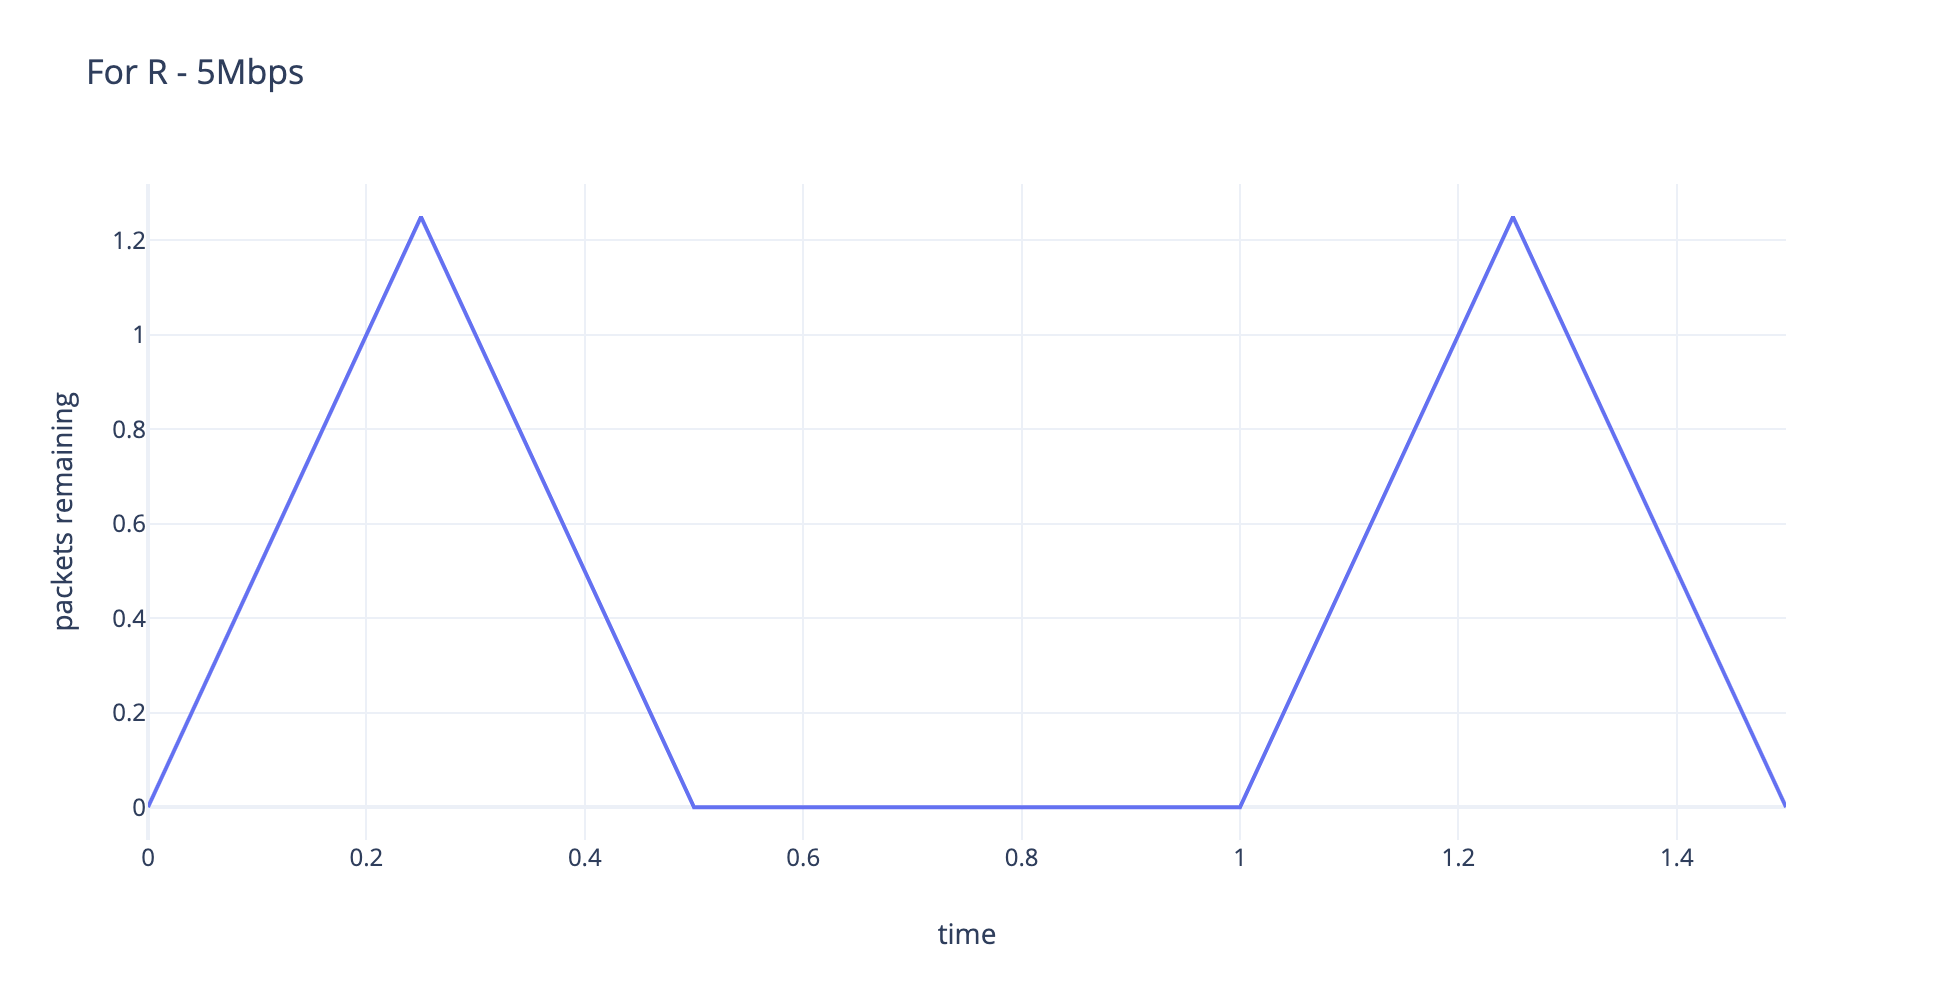
\includegraphics[width=0.75\columnwidth]{r_5.png}
    \end{center}
}
\end{homeworkSection}

\begin{homeworkSection}{(b)}
\problemAnswer{
    We could avoid buffer from growing by passing the incoming traffic received at the end of the period. \\
    As T=1s, \\
    From 0 to T/4s, $\frac{1}{4} * 10 = 2.5MBits$ is received.
    In order to avoid queuing, we must use a bandwidth of 2.5Mbps or above to transfer all the data received. 
}
\end{homeworkSection}

\begin{homeworkSection}{(c)}
\problemAnswer{
At any given time, the remaining queue size is 
\[
Q = 
\begin{cases}
  (10 - R)t & t \in \left[ 0, 1/4\right] \\
  max(2.5 - Rt, 0) & t \in \left( 1/4, 1\right)
\end{cases}
\]

Average delay of all bits is given using, \\
\begin{align*}
    D(R) & = \frac{1}{4} \int_{0}^{\frac{1}{4}} \frac{(10 - R)t}{R}dt \\
    &= \frac{10 - R}{8R}
\end{align*}
}
\end{homeworkSection}

\begin{homeworkSection}{(d)}
\problemAnswer{
The time required for the queue to be empty is 
\begin{align*}
    \frac{1}{4} (10) - Rt_0 & = 0\\
    2.5 - Rt_0 & = 0\\
    t_0 &= \frac{2.5}{R}
\end{align*}

Average buffer occupancy L(R) as a function of R is given using

\begin{align*}
    L(R) &= \int_{0}^{t_0} q(t) dt\\
    &= \int_{0}^{\frac{1}{4}} (10 - R)tdt + \int_{\frac{1}{4}}^{t_0} (2.5  - Rt)dt\\
    &= \frac{2.5}{R} \left(\frac{10 - R}{8}\right)
\end{align*}
}
\end{homeworkSection}

\begin{homeworkSection}{(e)}
\problemAnswer{
As $\lambda = 2.5Mbps$

\begin{align*}
   \mbox{As } L(R) &= \frac{2.5}{R} \left(\frac{10 - R}{8}\right) \\
    &= \lambda D(R)
\end{align*}
}
\end{homeworkSection}
\end{homeworkProblem}

%----------------------------------------------------------------------------------------
\pagebreak

\begin{homeworkProblem}
    \begin{homeworkSection}{(a)}
    \problemAnswer{
        A Circuit-switched network would be more suitable in this since the data transmitted is small, fixed and does not occur in burst. Also, the data would be transmitted for longer session hence a steady connection is needed.
    }
    \end{homeworkSection}
    
    \begin{homeworkSection}{(b)}
    \problemAnswer{
        Since the total sum of application data rates is less than the capacities of each and every link, no congestion control is needed as there would be little to no queuing. Hence no congestion is required as the link capacities are more than the data transferred.
    }
    \end{homeworkSection}
\end{homeworkProblem}

%----------------------------------------------------------------------------------------
\pagebreak

\begin{homeworkProblem}
    \begin{homeworkSection}{(a)}
    \problemAnswer{
        \begin{align*}
        \mbox{Total user} &= \frac{
                        \mbox{Transmission rate of link}
                    }{
                        \mbox{Transmission rate required by the user}
                    }\\
                    & = \frac{3000Kbps}{150Kbps}\\
                    & = 20 \mbox{ users}
        \end{align*}
    }
    \end{homeworkSection}
    
    \begin{homeworkSection}{(b)}
    \problemAnswer{
        Probability that the user is transmitting is 10/100 (since 10\% are active at a time) = 0.1
    }
    \end{homeworkSection}
    
    \begin{homeworkSection}{(c)}
    \problemAnswer{
        \begin{align*}
            P(n) &= C^N_n \left( P\right)^n\left(1 - P \right)^{N - n}\\
            &= C^{120}_n \left( 0.1 \right)^n\left(0.9 \right)^{120 - n}
        \end{align*}
    }
    \end{homeworkSection}
    
    \begin{homeworkSection}{(d)}
    \problemAnswer{
    Probability that 21 or more user are transmitting is given using 
        \begin{align*}
            P(>=21) &= 1 - P(<21)\\
            & = 1 - \left[P(0) + P(1) + P(2) + P(3) ... P(20)\right]\\
            & = 1 - \sum_{n = 0}^{20} C^{120}_n \left( 0.1 \right)^n\left(0.9 \right)^{120 - n}
         \end{align*}
    }
    \end{homeworkSection}
\end{homeworkProblem}


%----------------------------------------------------------------------------------------
\pagebreak

\begin{homeworkProblem}
    \begin{homeworkSection}{(a)}
    \problemAnswer{
    Total delay = Queuing delay + transmission delay
        \begin{align*}
            &= \frac{IL}{R(1 - L)} + \frac{L}{R}\\
            &= \frac{L}{R} \frac{1}{1 - I}
        \end{align*}
    }
    \end{homeworkSection}
    
    \begin{homeworkSection}{(b)}
    \problemAnswer{
        Let $x = \frac{L}{R}$\\
        Therefore total delay $F(x)$ is given by the following equation
        
        \begin{align*}
            & = \frac{L}{R} \frac{1}{1 - I} \\
            & = \frac{L}{R} \frac{1}{1 - a \frac{L}{R} }\\
            &= \frac{x}{1 - ax}
        \end{align*}
        \begin{center}
            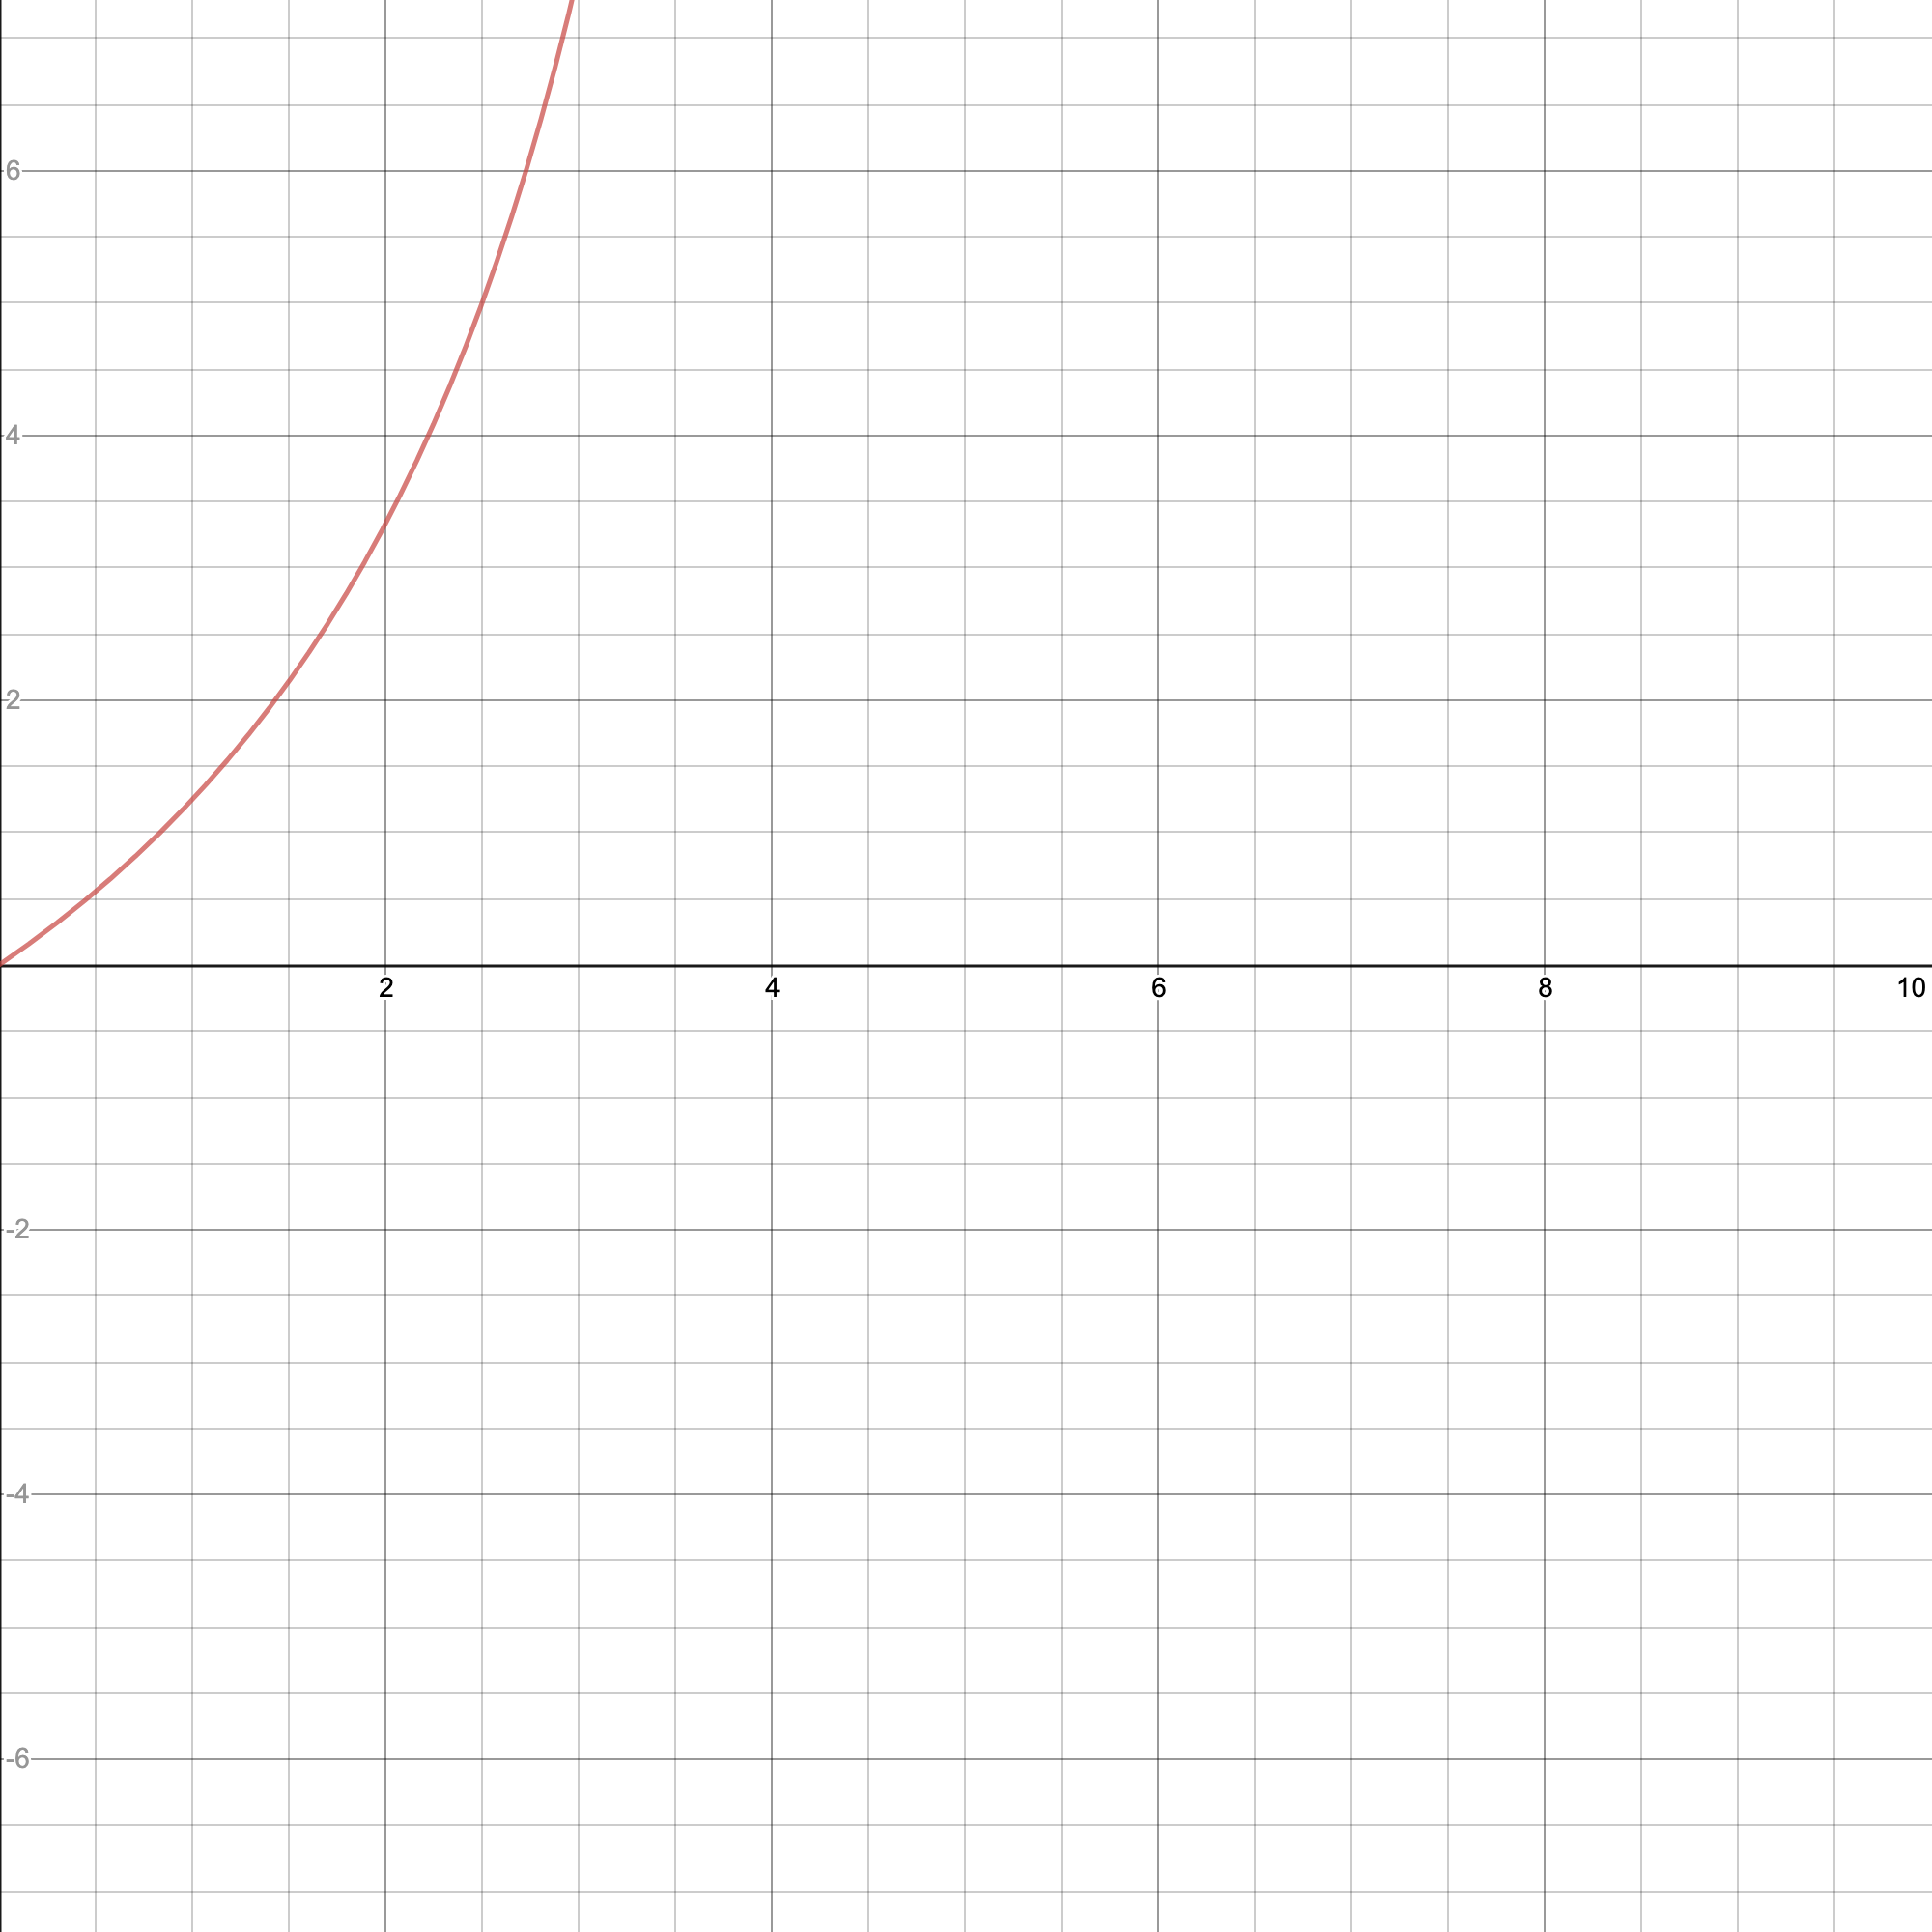
\includegraphics[width=0.75\columnwidth]{graph.png}
        \end{center}
        It is clear that as x $\rightarrow$ $\frac{1}{a}$, delay goes to infinity and when x $\rightarrow$ 0, delay goes to 0
    }
    \end{homeworkSection}
\end{homeworkProblem}



%----------------------------------------------------------------------------------------
\pagebreak

\begin{homeworkProblem}
    \begin{homeworkSection}{}
    \problemAnswer{
    As per Wikipedia,\\
    Total packets = Buffer packets + transmitted packet \\
        N = 10 \\
        
        As, 
        \begin{align*}
            N &= a * d \\
            10 &= a * (d_{queue} + d_{trans}) \\
            11 & = a * (0.01 + 0.01)\\
            a & = 500 \mbox{ packets/sec}
        \end{align*}
    As per textbook,\\
        Total packets = Buffer packets + transmitted packet \\
        N = 10 +  1 \\
        
        As, 
        \begin{align*}
            N &= a * d \\
            10 + 1 &= a * (d_{queue} + d_{trans}) \\
            11 & = a * (0.01 + 0.01)\\
            a & = 550 \mbox{ packets/sec}
        \end{align*}
        \textbf{The real ambiguity lies with respect to value of N}
    }
    \end{homeworkSection}
\end{homeworkProblem}



%----------------------------------------------------------------------------------------
\pagebreak

\begin{homeworkProblem}
    \begin{figure}
        \begin{center}
            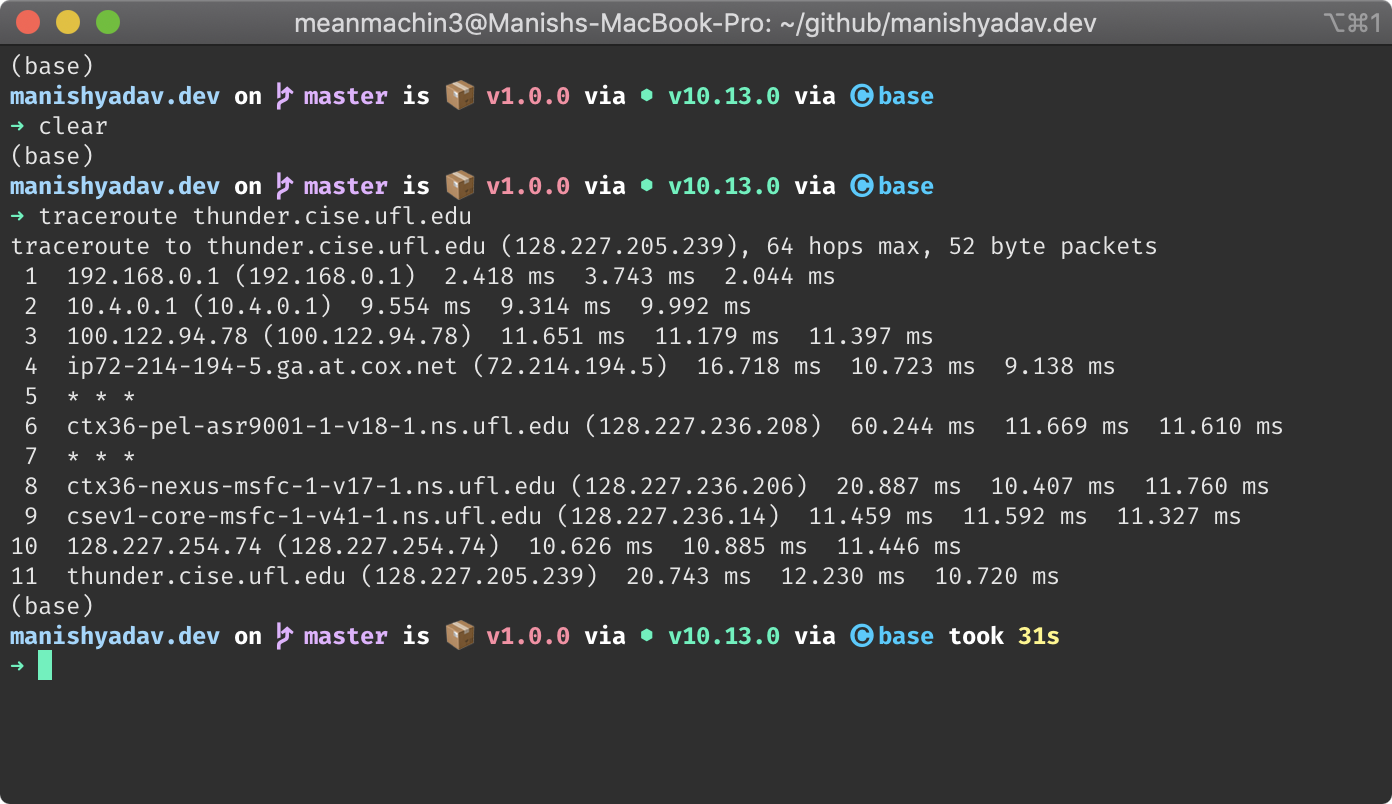
\includegraphics[width=0.75\columnwidth]{tr_1.png}
            \caption{traceroute from desktop to thunder.cise.ufl.edu 4 am}
            \vspace{2mm}
            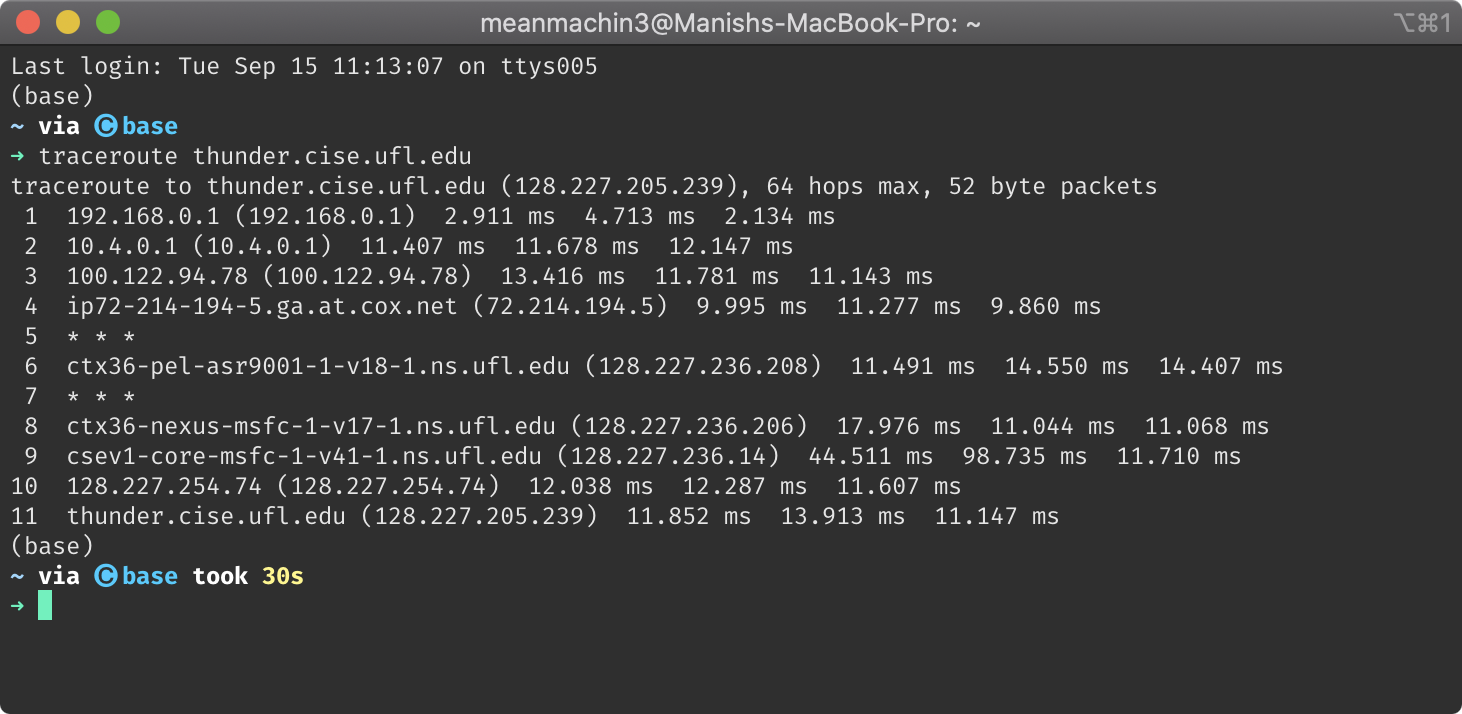
\includegraphics[width=0.75\columnwidth]{2.png}
            \caption{traceroute from desktop to thunder.cise.ufl.edu 11 am}
            \vspace{2mm}
            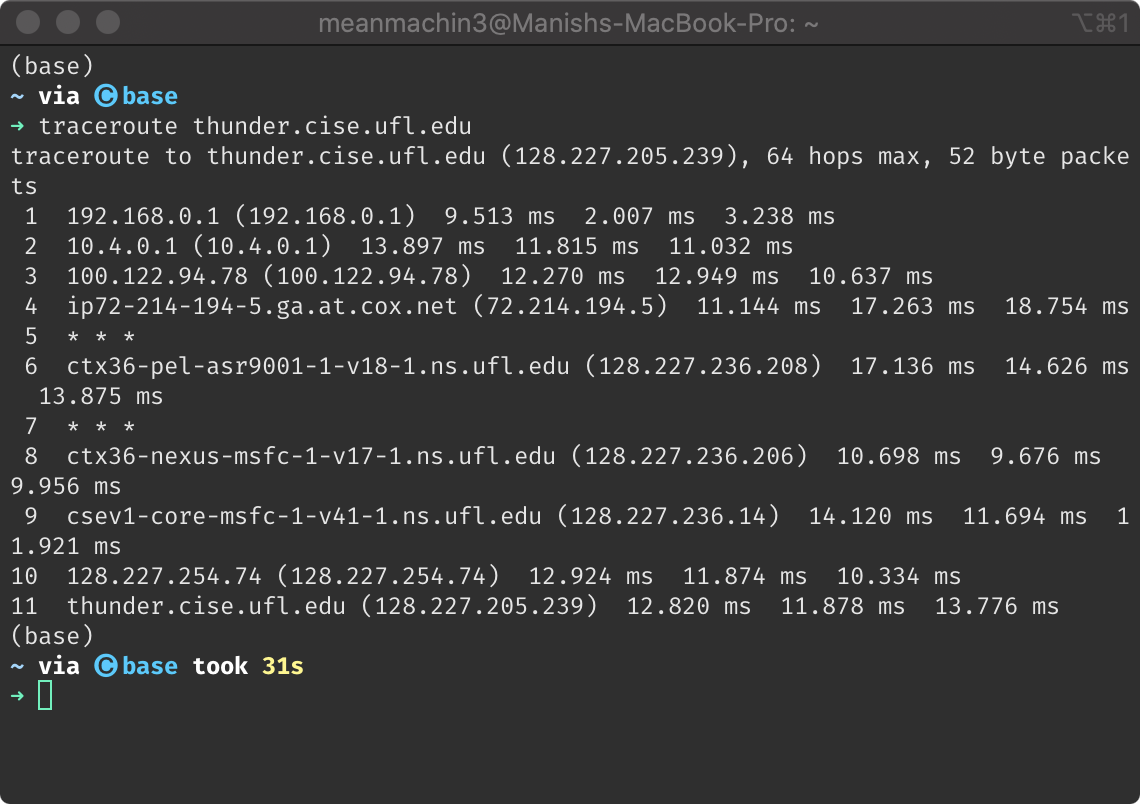
\includegraphics[width=0.75\columnwidth]{3.png}
            \caption{traceroute from desktop to thunder.cise.ufl.edu 2 pm}
        \end{center}
    \end{figure}
    \begin{homeworkSection}{(a)}
    \problemAnswer{
        The average of round trip delay is 15.138 ms, 12.673 ms, 11.881 ms and standard deviation is 3.982 ms, 0.888 ms, 1.351 ms.
    }
    \end{homeworkSection}
    \begin{figure}
        \begin{center}
            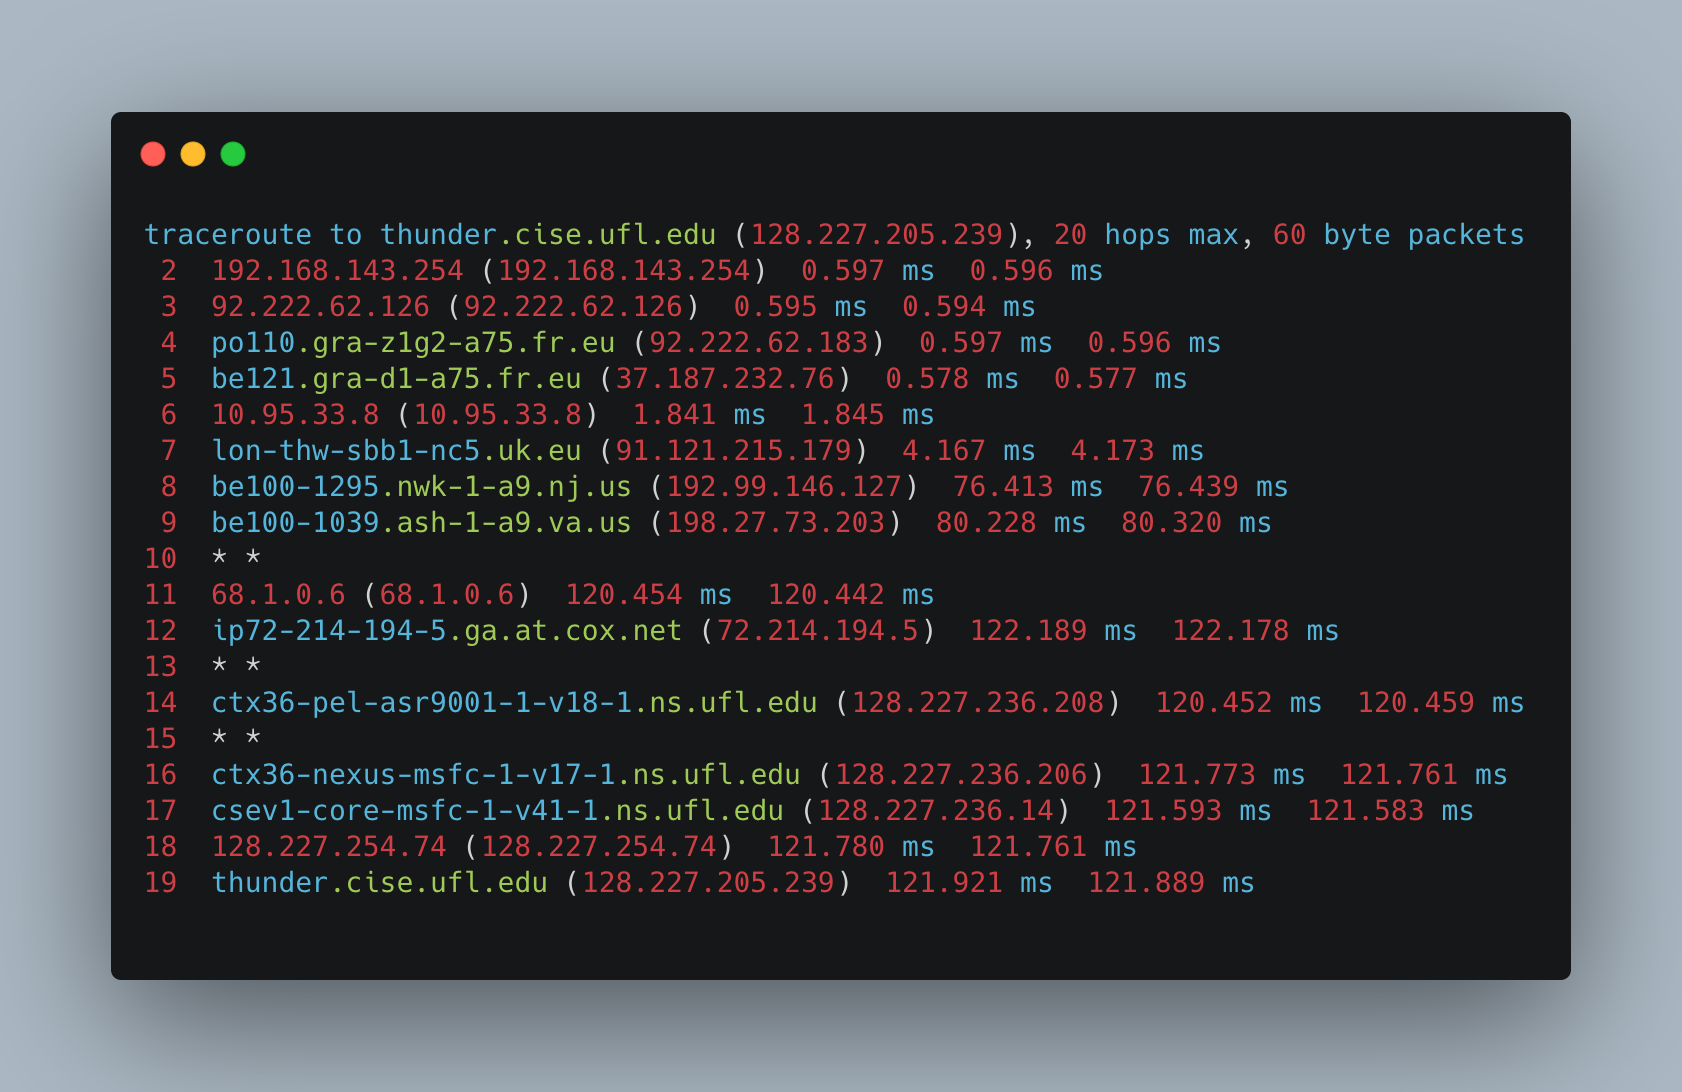
\includegraphics[width=0.75\columnwidth]{fr_1.png}
            \caption{traceroute from france to thunder.cise.ufl.edu 8 am}
            \vspace{2mm}
            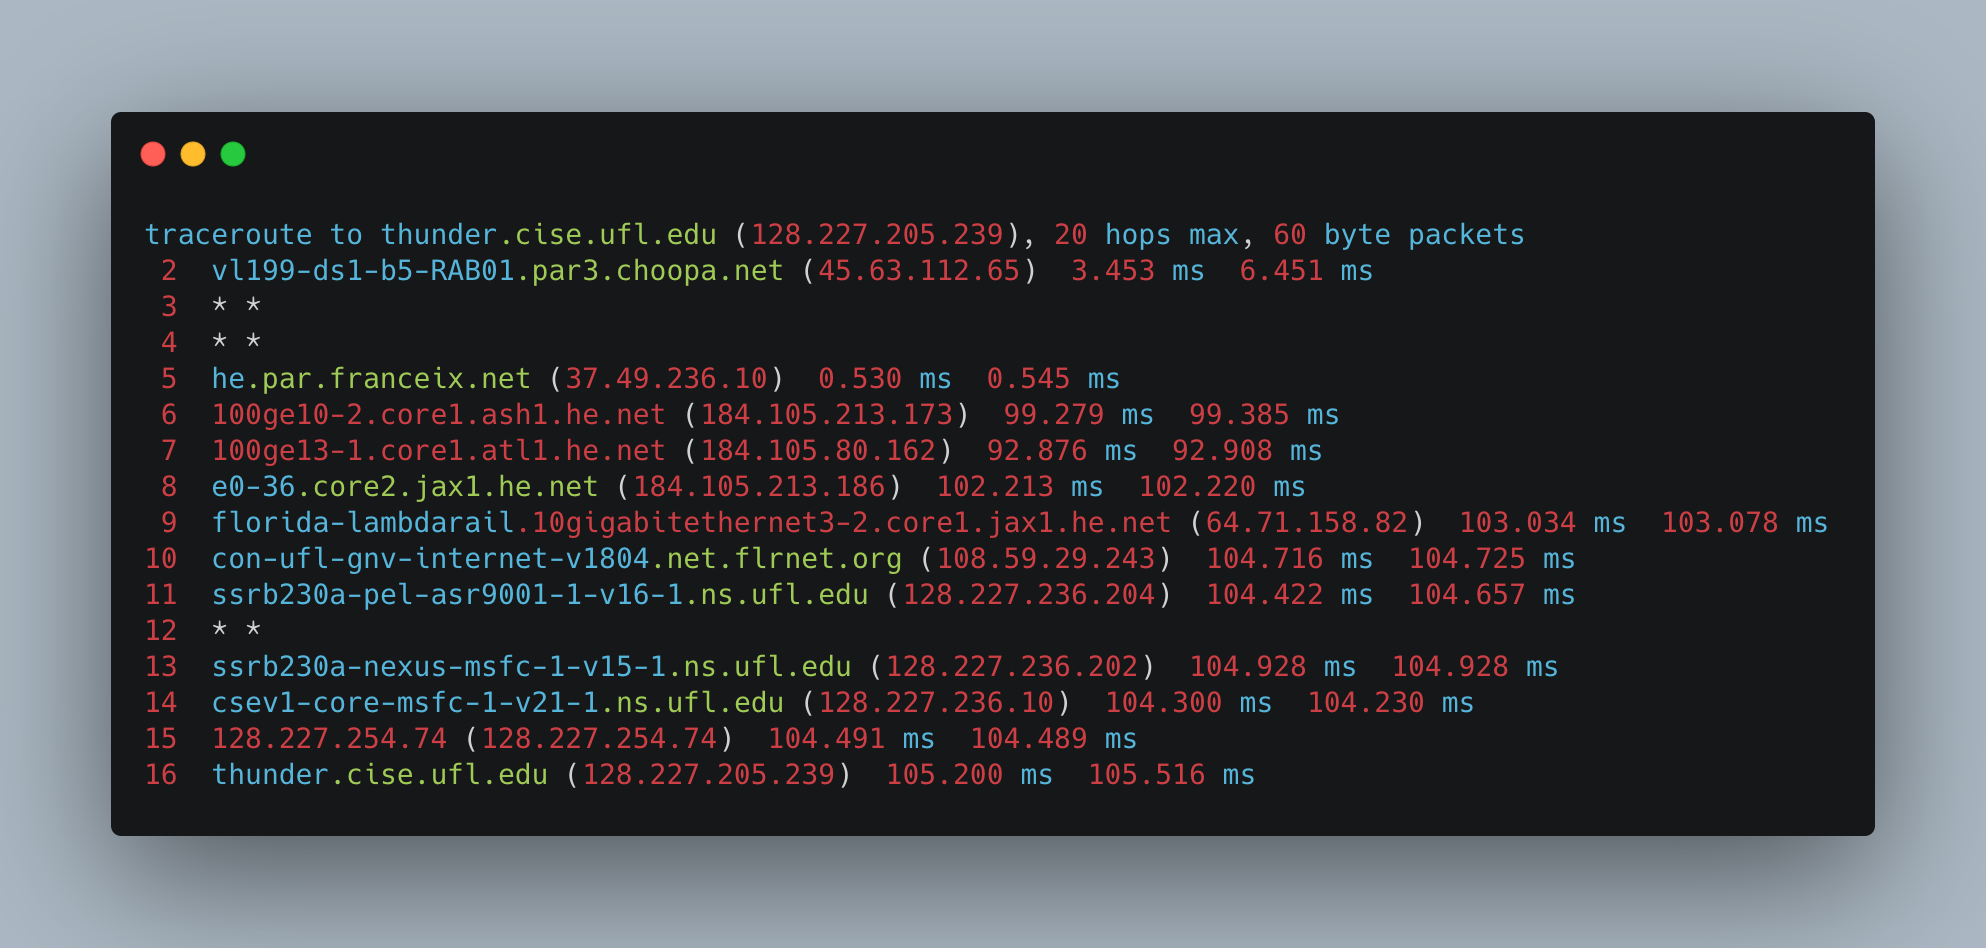
\includegraphics[width=0.75\columnwidth]{fr_2.png}
            \caption{traceroute from france to thunder.cise.ufl.edu 12 pm}
            \vspace{2mm}
            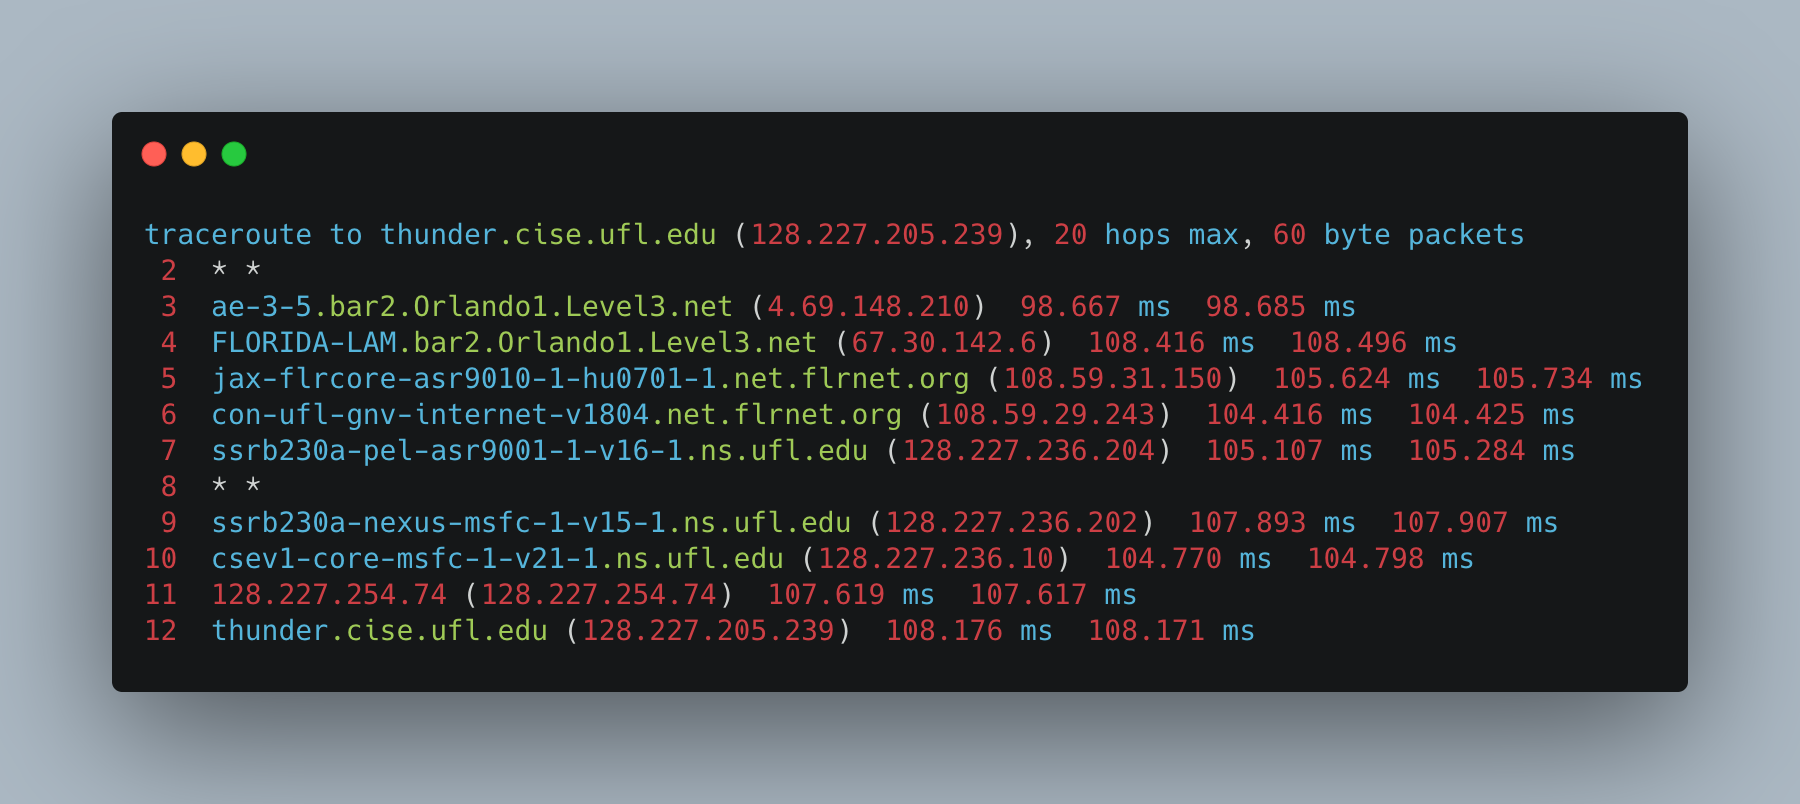
\includegraphics[width=0.75\columnwidth]{fr_3.png}
            \caption{traceroute from france to thunder.cise.ufl.edu 6 pm}
        \end{center}
    \end{figure}
    \begin{homeworkSection}{(b)}
    \problemAnswer{
        The traceroute between my laptop and thunder.cise.ufl.edu has 12 routers. There was no change in path.
    }
    \end{homeworkSection}
    
    \begin{homeworkSection}{(c)}
    \problemAnswer{
        There were a total of 3 ISP in traceroute between my laptop and thunder.cise.ufl.edu. 
        There is a spike whenever there is change of ISP i.e at the peering interfaces
    }
    \end{homeworkSection}
    
    \begin{homeworkSection}{(d)}
    \problemAnswer{
       The average of round trip delay is 111.765 ms and 111.858 ms and standard deviation is 7.282 ms and 7.174 ms.\\
       The traceroute from france and thunder.cise.ufl.edu had varying amount of routers (12-19). There was change in path.
       There were a varying amount of ISP(4-6) in traceroute between france and thunder.cise.ufl.edu.
       There is a spike whenever there is change of ISP i.e at the peering interfaces
    }
    \end{homeworkSection}

\end{homeworkProblem}

%----------------------------------------------------------------------------------------
\pagebreak

\begin{homeworkProblem}
    \begin{homeworkSection}{(a)}
    \problemAnswer{
        \begin{align*}
            d_{prop} = \frac{20000 * 1000}{2.5 * 10^8} = 0.08 s
        \end{align*}
         Bandwidth-delay product = $R * d_{prop}$ \\
         = $2 * 10^6 * 0.08$ \\
         = $16 * 10^4$
         
    }
    \end{homeworkSection}
    
    \begin{homeworkSection}{(b)}
    \problemAnswer{
         The bandwidth delay product is the maximum number of bit that can be in the link. Since we are transmitting $80 * 10 ^4$ and the bandwidth delay product is $16 * 10^4$. Therefore at given time the maximum bit in the link would be $16 * 10^4$
    }
    \end{homeworkSection}
    
    \begin{homeworkSection}{(c)}
    \problemAnswer{
         The bandwidth delay product is the maximum number of bit that can be in the link.
    }
    \end{homeworkSection}
    
    \begin{homeworkSection}{(d)}
    \problemAnswer{
         The width of the bit in the link is given using
         \begin{align*}
            \frac{20000 * 1000}{16 * 10^4} = 125m
        \end{align*}
        It is indeed larger than football field of 100 yards (91.44 m)
    }
    \end{homeworkSection}
    
    \begin{homeworkSection}{(e)}
    \problemAnswer{
         Width of bit is given using the following
         \begin{align*}
            & = \frac{m}{R * d_{prop}} \\
            &= \frac{m}{R * \frac{m}{s}}\\
            &= \frac{s}{R}
        \end{align*}
    }
    \end{homeworkSection}
\end{homeworkProblem}


\end{document}
%----------------------------------------------------------------------------------------
%	DONE
%----------------------------------------------------------------------------------------
